%!TEX root = ../../thesis.tex

\section{Continuous set of hypothesis}
\label{chapter:limitations:continuoushypothesis}

\question{How to leverage from the finite set of hypothesis constraint?}

In order to make the learning problem tractable, it was assumed that the robot learner knows that the task to be learnt can be approximated by one task among a pre-defined set of tasks. Indeed, without constraining the space of possible tasks, an infinite number of task may explain the particular teaching data received by the robot. In practice, the number of pre-defined tasks in the experiment was still relatively large, allowing a certain level of flexibility. Yet, it would be highly desirable to extend the possibility to deal with continuous task representation, allowing potentially infinite spaces of tasks. 

A potential avenue to address this is to constrain search through a combination of regularization and particle filter approaches. In the following of this section, we present a simple particle filter based algorithm that allow an agent to identify a task from unlabeled instruction and considering an infinite set of hypothesis. The agent evolve in a 2 dimensional continuous state and should identify which one of the infinite amount of possible state it should reach.

\subsection{World and task}

We consider an agent living in a 2 dimensional continuous space bounded between 0 and 1 in both dimension. A teacher is providing indication about the orientation of the goal state compared to the robot state by drawing some patterns on a tablet. Those direction can only be selected among of the four cardinal directions that are the directions of north, east, south, and west. The teacher wants the robot to reach a particular state, that can be any position in the continuous 2 dimensional space. The robot is able to teleport itself to any location of the space to receive a new indication.

We still consider a strong a priori knowledge on the space of task, which is that there is only one goal state. This is a very strong a priori regularization on the complexity of the problem. Considering there could be several goal positions, depending for example on the current position of the agent, would increase dramatically the search space; it would then be likely that many hypothesis of different complexity would explain perfectly the observed data. In such case a rule for regularizing the hypothesize task solution would be needed.

\subsection{Interaction frame}

We use the cardinal direction frame define in section~\label{chapter:limitations:framegeneric} in Equation~\ref{eq:cardinalframe} with $\alpha = 0.01$. In this frame, the user provide an information about the cardinal direction of the goal state with respect the current agent position. The agent does not have to know how to reach a state to interpret the signal according to that state as only the absolute direction matters.

\subsection{Finger movements datasets}

We will present results using two different datasets made of finger movements performed on a tablet. 

Our first dataset shown in Figure~\ref{fig:fingerdatasetdirection} is build from a user generating directional trajectories starting from the center of the tablet and going toward the edges of the tablet. We considered four different movement, one toward each edges, representing the four cardinal directions that are the directions of north, east, south, and west. 

\begin{figure}[!ht]
\centering
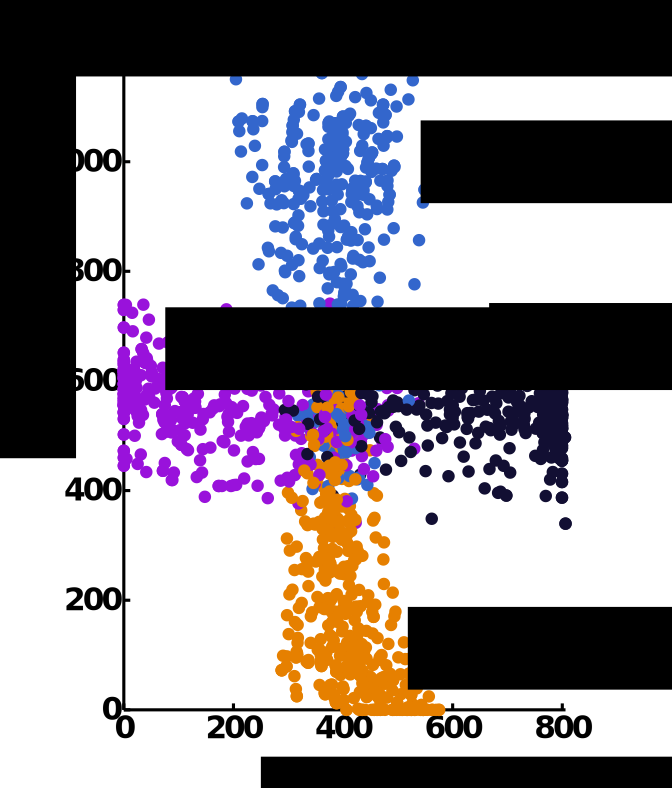
\includegraphics[width=\signalwidth\columnwidth]{\visualspdf/worlds_and_datasets/finger_signals_color.pdf}
\caption{N}
\label{fig:fingerdatasetdirection}
\end{figure} 

Our second dataset shown in Figure~\ref{fig:fingerdatasetsigns} is build from a user drawing The cardinal letters (N, S, W, and E) in the middle of the tablet.

\begin{figure}[!ht]
\centering
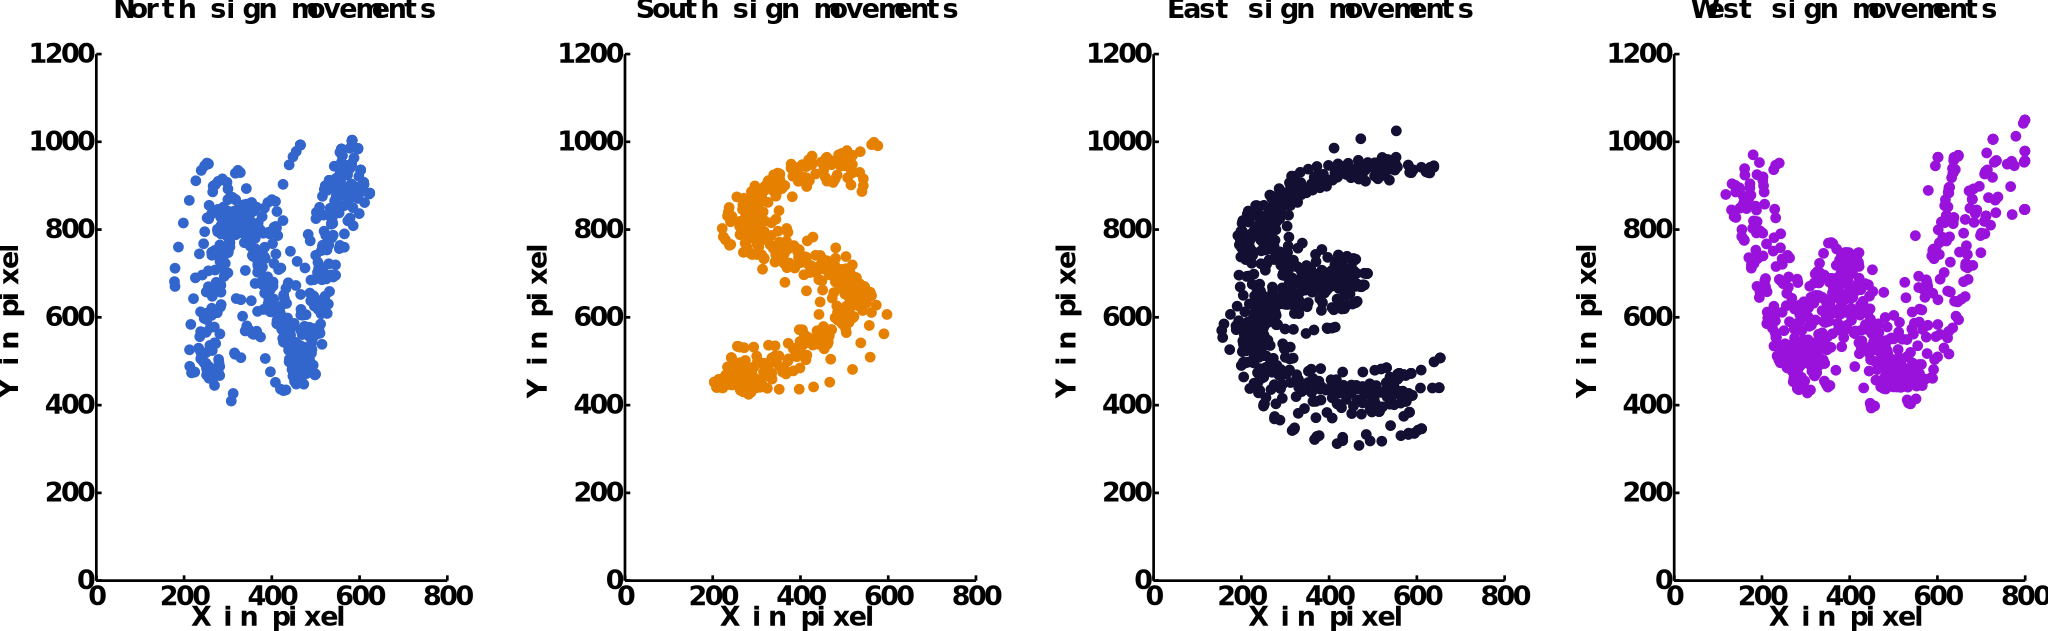
\includegraphics[width=\columnwidth]{\visualspdf/worlds_and_datasets/finger_signals_color_signs.pdf}
\caption{N}
\label{fig:fingerdatasetsigns}
\end{figure} 

To represent those trajectories, our feature vector is composed of 11 dimensions, where dimensions encodes:
\begin{itemize}
   \item The start X and Y positions (2 features)
   \item The end X and Y positions (2 features)
   \item The delta position between start and end position for X and Y coordinate (2 features)
   \item The median X and Y positions (2 features)
   \item The distance between start and end position (1 feature)
   \item The total distance traveled by the finger (1 feature)
   \item The average speed of the finger (1 feature)
\end{itemize}

Using this representation we achieve 100 percent accuracy on the directional movements dataset and 99 percent accuracy on the cardinal signs dataset, using a simple Gaussian classifier with one Gaussian per class.

We remind that the direction of shape of each movement has no a priori meaning for the robot. For example, in our simulation we may use the ``W'' sign signals to mean the goal state is north to the agent position.

\subsection{Evaluating task likelihood}

As there is an infinity of possible goal state, the agent can not estimate the probability of all possible task in parallel. We will rely on a particle filter based approach \cite{gordon1993novel,doucet2009tutorial,thrun2002particle}. The main idea consist of sampling a finite number of task and compute a confidence measure for each of those task. Given the ranking between them, we will apply a resample step which consist of keeping some of the best task and sample a bunch of new ones. More details are provided in next subsection~\ref{chapter:limitations:continoushypothesis:particlefilter}, we present in this subsection how we estimate the probability of each sampled task.

Our algorithm, as presented so far, was cumulatively accumulating evidence for each task and updated the likelihood of each task on a step by step basis. However for this experiment, as we the task hypothesis are changing step after step, we can not update the likelihood of each task on a step by step basis, as described in Equation~\ref{eq:matchingfiltercrossvalidation}. This approach allowed us to reduce the computational cost of our algorithm so as to be able to run our experiments in a reasonable amount of time. A possible option would be to use Equation~\ref{eq:matchingcrossvalidation}, but we would have to train a huge amount of classifier each step (100000 classifiers after 200 steps in our experiments).

We selected an other option which rely on sampling different classifier from a meta-classifier, which allow us to generate classifiers at a low computational cost. Then given many classifiers for each task, we will compare the likelihood predicted by those classifiers and rank the task by a statistical test on the classifier evaluation. We describe each step of this process in the following paragraph.

The first step is to compute a ``meta'' model which encodes a distribution of probability on the classifier parameters, i.e. which encodes a probability distribution over the mean and covariance of each class. To do so, and given that we are using multivariate normal distribution, we use a noninformative (Jeffrey's) prior \cite{gelman2003bayesian} to estimate the probability distribution over the means and covariances:

\begin{eqnarray}
p(\mu_l|D) & = & t_{n-d}(\mu| \bar{x}_l, \frac{S_l}{n(n-d)})
\label{eq:jeffreysmean}
\end{eqnarray}

\begin{eqnarray}
p(\Sigma_l|D) & = & IW_{n-1}(\Sigma_l | S_l)
\label{eq:jeffreyscov}
\end{eqnarray}

where $\bar{x}_l$ and $S_l$ respectively represents the ML estimates of the mean and covariance for each class $l$ based on the dataset $D$, $n$ is the number of signals, and $d$ is the dimensionality of a signal feature vector.
$\mu_l$ and $\Sigma_l$ are the posterior estimates of the mean and covariance given the noninformative prior. $IW$ denotes an Inverse Wishart function which is the multidimensional generalization of the inverse Gamma, it represents a probability distribution on covariance matrix.

This ``meta'' model encodes the distribution of probability on the classifier parameters. Given this model we can sample, for very low computational cost, a multitude of possible QDA classifiers by sampling a mean and covariance for each class. The more we have data to fit our model, the less uncertainty remains and the less variability will be observed in the generated classifiers. 

In our experiment we will sampled 20 classifiers per task. For each sampled set of classifiers, we compute the probability value (i.e. the normalized likelihood) of each task. As a results we have 20 estimations of the probability of each task. We will consider one task as the best one once one of the task as significantly better probabilities than all the others. 

To do so we model our 20 probability estimates for each task by a normal distribution, and denote as $\mu_{\xi_t}$ and $\sigma_{\xi_t}$ the associated maximum likelihood estimates of the mean and variance. To compare two distributions, we compute the probability that one sample from the  Gaussian associated to one task has higher value than one sample from the Gaussian associated to the other task. To do so we compute the normal difference distribution between the two models of each task probabilities. The resulting model is also a normal distribution with mean and variance as follows:
%
\begin{eqnarray}
\mu_{\xi_t - \xi_u} = \mu_{\xi_t} - \mu_{\xi_u} 
\label{eq:meandiffgaussian}
\end{eqnarray}
%
\begin{eqnarray}
\sigma^2_{\xi_t - \xi_u} = \sigma^2_{\xi_t} + \sigma^2_{\xi_u}
\label{eq:variancediffgaussian}
\end{eqnarray}

Finally we compute the probability than one sample from that class as a value above zero. This is simply $1 - \Phi(\mu_{\xi_t - \xi_u}, \sigma^2_{\xi_t - \xi_u})$, with $\Phi(\mu_{\xi_t - \xi_u}, \sigma^2_{\xi_t - \xi_u})$ the cumulative normal distribution associated to the normal distribution of mean $\mu_{\xi_t - \xi_u}$ and variance $\sigma^2_{\xi_t - \xi_u}$. Then, as for equation~\ref{eq:probapairwise} we take as probability for the task  $\xi_t$ the minimum of the pairwise comparison with all other tasks $\xi_u$ with $u~\in~\{1, \ldots, T\} \smallsetminus \{t\}$.


We illustrate this process in Figure~\ref{fig:normaldifferencedistribution}. 20 samples were generated randomly to simulate some estimates for two task hypothesis and model their respective distribution using normal distribution (see Figure~\ref{fig:normaldifferencedistribution:data}). Finally we compute the probability that a sample from the distribution with highest mean has higher value than a sample from the distribution with lowest mean. We use Equations~\ref{eq:meandiffgaussian}~and~\ref{eq:variancediffgaussian} to compute the mean and variance of the normal difference distribution between the two distributions, The area under curve from 0 to +Inf is our probability measure.

\begin{figure}[!ht]
\centering
    \begin{subfigure}[b]{\columnwidth}
        \centering
        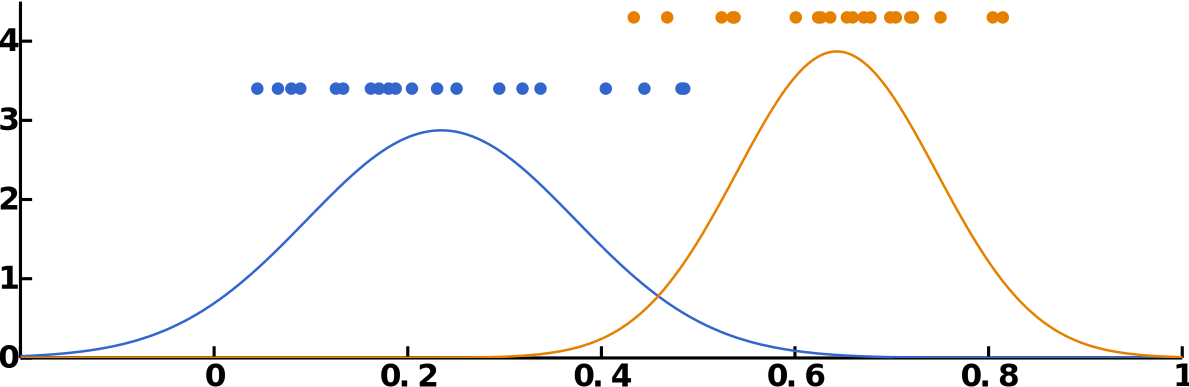
\includegraphics[width=\columnwidth]{\visualspdf/normal_diff/data.pdf}
        \caption{Normal distribution fitted from the estimated values of two hypothesis. On top are the 20 samples associated to each hypothesis. The orange distribution has a mean of 0.71 and a standard deviation of 0.17. The blue distribution has a mean of 0.23 and a standard deviation of 0.16.}
        \label{fig:normaldifferencedistribution:data}
    \end{subfigure}
    \begin{subfigure}[b]{\columnwidth}
        \centering
        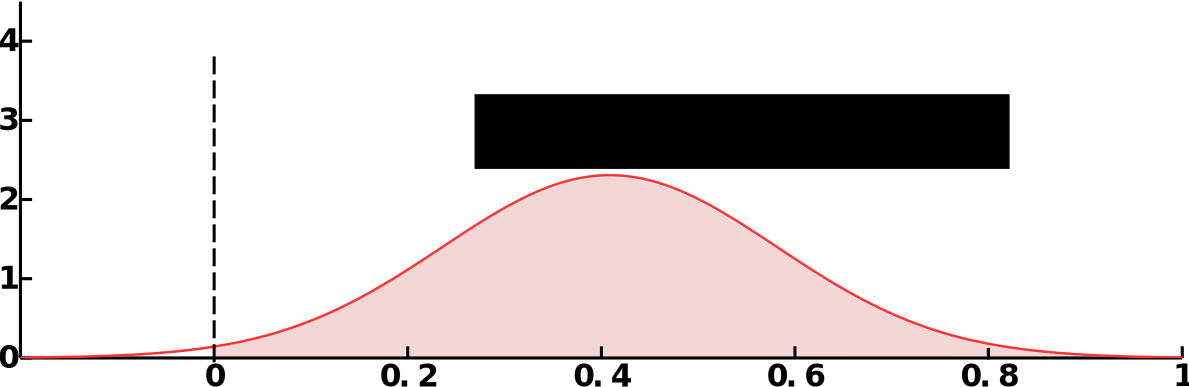
\includegraphics[width=\columnwidth]{\visualspdf/normal_diff/pdfDiff.pdf}
        \caption{Normal difference distribution between the two distribution of Figure~\ref{fig:normaldifferencedistribution:data} (the orange one minus the blue one). Mean is 0.48 and standard deviation is 0.23. From this distribution we estimate the probablity that a sample has a value above zero, in this example it would be 0.99.}
        \label{fig:normaldifferencedistribution:pdf}
    \end{subfigure}
    \begin{subfigure}[b]{\columnwidth}
        \centering
        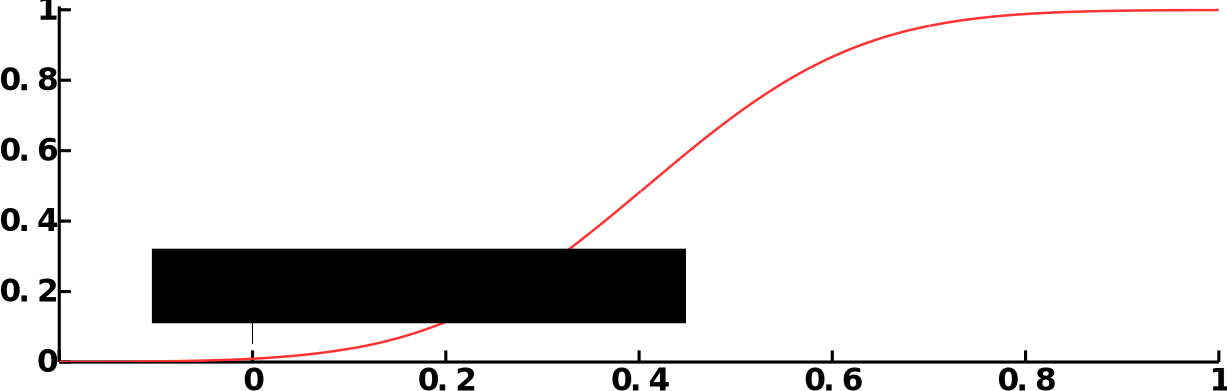
\includegraphics[width=\columnwidth]{\visualspdf/normal_diff/cdfDiff.pdf}
        \caption{Cumulative normal distribution of the Gaussian in Figure~\ref{fig:normaldifferencedistribution:pdf}.}
        \label{fig:normaldifferencedistribution:cdf}
    \end{subfigure}
\caption{The procedure used to estimate the probability that one hypothesis generates better classifiers than an other.}
\label{fig:normaldifferencedistribution}
\end{figure}

There is several weaknesses in this approach and we note that modeling a distribution on the interval [0, 1] using a normal distribution is not appropriate. Using a beta distribution would have been more suitable but we could not find an analytical solution to the difference between two beta distributions. However, we tried to use more standard statistical test, such as the one tailed Student's t-test or the Welch's t-test, but the results were not satisfying as those tests only check whether or not the means of the distributions are equals.

Note that it would seem more straightforward to directly compute the marginal probability distribution of Equation~\ref{eq:prior} which integrates over the all distribution of parameters; and use this for our likelihood estimates of Equation~\ref{eq:matchingoverfitting}. Here we tried to get a measure of confidence on top of our likelihood estimates. This is why we generate several classifiers, test their performances and measure the probability that one set of classifiers is on average better that an other set of classifiers. To do so we model the distribution of performances of a set of classifiers by a normal distribution; and compute the probability that a sample drawn from the distribution associated to one set of classifiers has higher value than one drawn from the distribution associated the an other set of classifiers.

\subsection{Task hypothesis selection and generation}
\label{chapter:limitations:continoushypothesis:particlefilter}

As there is an infinity of possible goal state, the agent can not estimate the probability of all possible task in parallel. We will rely on a particle filter based approach \cite{gordon1993novel,doucet2009tutorial,thrun2002particle}. The main idea consist of sampling a finite number of task and compute a confidence measure for each of those task. Given the ranking between them, we will apply a resample step which consist of keeping some of the best task and sample a bunch of new ones.

There is many parameters that will influence the performance of such an algorithm. We can change the number of task sampled, the criteria for selecting the task(s) that stay in the pool from one step to another, and we can change the method used to sample new task. 

As this is an exploratory experiment, we will restrict our analysis to the influence of the method used to resample the pool of task hypothesis and consider either a random or an active strategy. In practice, we will consider a pool of 50 hypothesis. Each step, we will keep the best hypothesis from the pool and replace the 49 others using one of the sampling strategies define next.

The random generation of task simply keeps the best hypothesis and generate 49 new tasks hypothesis randomly.

Our active task generation method simply selects new task around the current best task hypothesis. To do so, we create a mixture of Gaussians which define the probability distribution used to sample the new tasks. This mixture model is composed of:
\begin{itemize}
\item  one fixed Gaussian at the center of the state space (i.e. $[0.5, 0.5]$), with a diagonal covariance matrix, where each value on the diagonal is equal to $0.1$, and have an associated weight of $0.2$. This Gaussian, which as quite spread covariance matrix, maintains a level of exploration in the task generation process.
\item a multitude of Gaussians, one at each location of the previous hypothesis positions (i.e. hypothesized task), whose associated weights are proportional to the probability associated to each task. The sum of the weights of those Gaussians behind 0.8, such as the sum of all mixture component weight is 1. All those Gaussians have a diagonal covariance matrix, where each value on the diagonal is equal to $0.01$. For computational purpose, each Gaussian had a minimal weight of $1e^{-6}$.
\end{itemize}
Note that the resulting distribution will be truncated as all the point generated outside of the boundaries of the space (i.e. between 0 and 1 for each dimension) will be translated to the closest position on the boundaries of the state space.

\subsection{Uncertainty based state sampling}

The agent can also control the next state to teleport to. As seen in chapter~\ref{chapter:planning}, actively controlling agent state important can lead to better performances. Indeed the state of the agent influences the signal sent by the teacher. 

We will compare two kind of active sampling, random and an uncertainty based method. The random method simply teleport the agent to a random position in the world. 

The active method rely again on a sampling method. At each step, we generate 1000 states randomly and compute the uncertainty associated to those states using the method described in chapter~\ref{chapter:planning} by Equation~\ref{eq:planning} and using up to 20 sampled signals from our history of interaction. For the next state, we select, among the 1000 points, the one that as higher uncertainty, and teleport the agent to that state in order to collect the next teaching signal.

\subsection{Results}

We will compare all four combinations of the methods described above \begin{inparaenum}[a)] \item random state and task selection (which we call ``random random''), \item random selection of next state and active task sampling (which we call ``random active''), \item uncertainty based selection of next state and random task selection (which we call ``uncertainty random''), and \item uncertainty based selection of next state and active task sampling (which we call ``uncertainty active''). \end{inparaenum}

We ran 100 simulated experiments for each method and each dataset. Each experiment lasted 200 iteration and started by 12 random steps such as to collect enough point to use Equation~\ref{eq:jeffreysmean}~and~\ref{eq:jeffreyscov} with our 11 dimensional signals.

\paragraph{Distance to goal state}

We first analyse the results using the directional finger movement dataset shown in Figure~\ref{fig:fingerdatasetdirection}. For each method, we compare the evolution of the distance between the best task hypothesis through iteration (the more probable according to our estimate) and the goal state (see Figure~\ref{fig:continuoustaskdistevolution}).

Only the combination of actively sampling new task and actively selecting new state based on their relative uncertainty as overall better performance than any other combination of our method. Those two method are complementary, to find a task hypothesis better than our previous best estimates, it is likely that it is close to the current best hypothesis. Our active task sampling method allow to explore close to our previous best estimates. However, now that we have some hypothesis located in a restricted area of the space, we need to sample state in very precise location to be able to differentiate them, which our uncertainty based state selection allow. This explain why using one of the two method alone do not reach the same performances as their combination.

\begin{figure}[!ht]
\centering
\includegraphics[width=0.62\columnwidth]{\imgpath/continuous_task/distEvolution.eps}
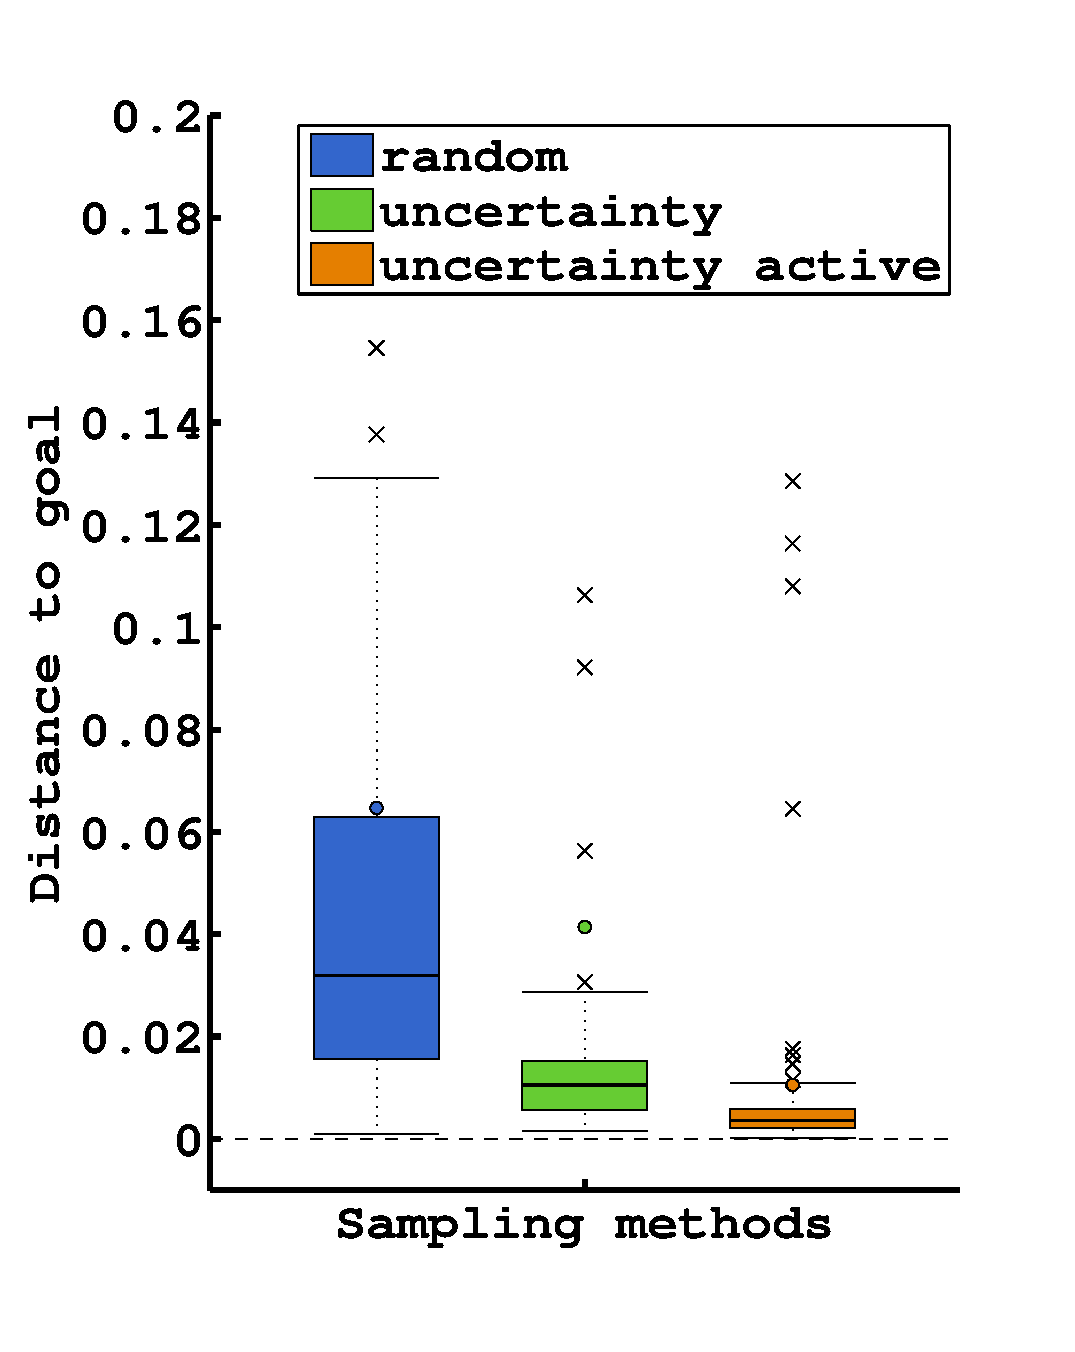
\includegraphics[width=0.37\columnwidth]{\imgpath/continuous_task/endDist.eps}
\caption{Evolution of the distance to target using the directional finger movement dataset shown in Figure~\ref{fig:fingerdatasetdirection}. On the left is the evolution of the distance of the best position hypothesis to the goal position (mean and standard error shown as shaded area). On the right is a box plot of the distance of the best position hypothesis to the goal position at the end of the 200 iterations. Actively sampling new task hypothesis as well as selecting new state based on our uncertainty estimation outperform allow to identify the target position with very high accuracy and low variance. Note that some distant outliers are not shown on the box plots for readability reasons.}
\label{fig:continuoustaskdistevolution}
\end{figure}

In Figure~\ref{fig:continuoustaskdistevolution} right, we compare the distribution of final distance between our best hypothesis and the true goal position. First note that the important difference between displaying our results in terms of mean and standard error or in terms of a box plot, which shows the median and the 25th and 75th percentile (you can see the mean value as a colored dot). Especially for the ``uncertainty random'' method, the visual impression of the performance of the methods differs. This is due to the outliers, where even a few values far away from the main group of point can ``push'' the mean away, the normal distribution assumption do not hold for presenting our results. In order to statistically compare the efficiency of our methods, we use the Mann-Whitney U-test \cite{mann1947test} which is a nonparametric test for equality of population medians of two independent samples. We will use the one tailed version to specifically test whether one population has greater performances than the other. There is no measurable statistical difference between the ``random random'' and ``random active'' methods ($p = 0.68$). The ``uncertainty random'' performances over ``random random'' ($p<1e^{-10}$) and ``random active'' ($p<1e^{-10}$) are highly significant. As well as the difference between the ``uncertainty active'' and ``uncertainty random'' difference in performance ($p<1e^{-10}$).

The results presented above where obtained using the directional finger movement dataset shown in Figure~\ref{fig:fingerdatasetdirection}. We now demonstrated how the same algorithm could handle different preferences of user finger gesture for cardinal direction indication. To do so we repeat the experiment with the cardinal sign dataset of Figure~\ref{fig:fingerdatasetsigns}.

\begin{figure}[!ht]
\centering
\includegraphics[width=0.62\columnwidth]{\imgpath/continuous_task/distEvo_signs.eps}
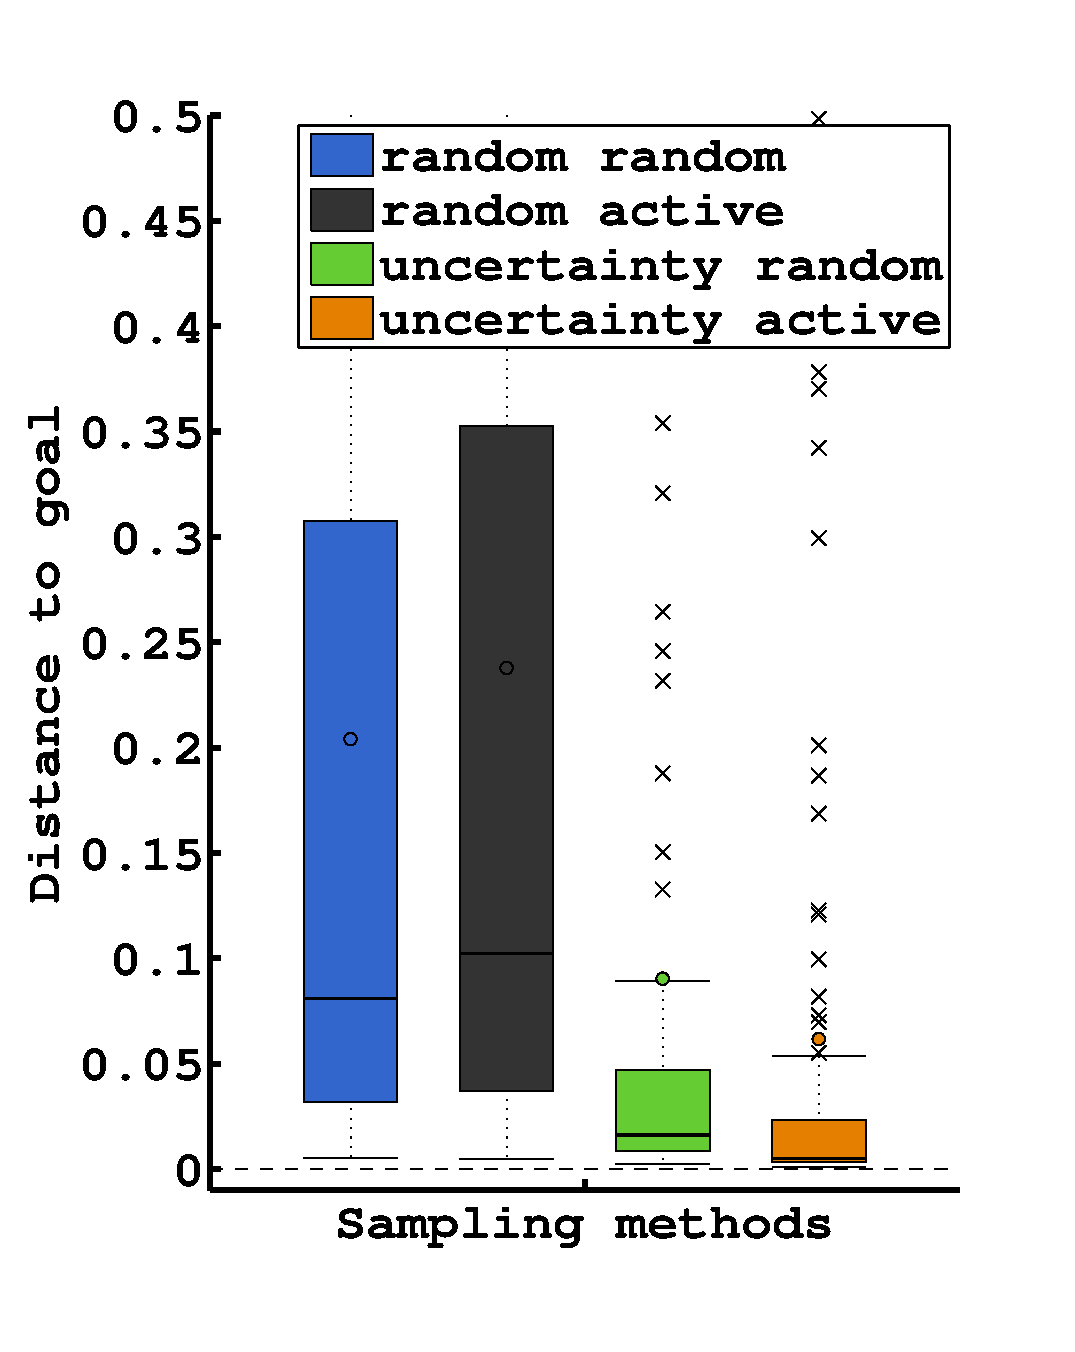
\includegraphics[width=0.37\columnwidth]{\imgpath/continuous_task/endDist_signs.eps}
\caption{Evolution of the distance to target using the cardinal signs finger movement dataset shown in Figure~\ref{fig:fingerdatasetsigns}. On the left is the evolution of the distance of the best position hypothesis to the goal position (mean and standard error shown as shaded area). On the right is a box plot of the distance of the best position hypothesis to the goal position at the end of the 200 iterations. Actively sampling new task hypothesis as well as selecting new state based on our uncertainty estimation outperform allow to identify the target position with very high accuracy and low variance. Note that some distant outliers are not shown on the box plots for readability reasons.}
\label{fig:continuoustaskdistevolution_signs}
\end{figure}

Figure~\ref{fig:continuoustaskdistevolution_signs} left shows the evolution of the distance between the best task estimates and the goal task. We observe a larger difference between random and uncertainty based selection of next state. This could be explained by the properties of the cardinal sign dataset, where the system must make use of all features to differentiate between classes which requires more evidence to be collected. For the directional finger movement dataset (Figure~\ref{fig:fingerdatasetdirection}), only two features (end position on X and Y axis) were enough to differentiate between all classes.

In Figure~\ref{fig:continuoustaskdistevolution_signs} right, we compare the distribution of final distance between our best hypothesis and the true goal position. There is no measurable statistical difference between the ``random random'' and ``random active'' methods ($p = 0.8687$). The ``uncertainty random'' performances over ``random random'' ($p<1e^{-10}$) and ``random active'' ($p<1e^{-10}$) are highly significant. As well as the difference between the ``uncertainty active'' and ``uncertainty random'' difference in performance ($p<1e^{-5}$).

Finally, we note that the final median distance between the best position estimation and the goal position are 0.0036 and 0.0051 for the directional movement and cardinal sign movement respectively. While this does not really matter, this difference is significant ($p< 1e^{-3}$). However it is important to project this results in the real word, it would mean that given a one meter square area, our agent is able to find the position the user has in mind with less that 5 millimeter error, half of the time and given 200 requests, but without knowing the signal to meaning mapping beforehand. Moreover, as we have seen with our two datasets (Figure~\ref{fig:fingerdatasetdirection} and Figure~\ref{fig:fingerdatasetsigns}), given our simple representation of the finger movements, a great variety of possible signals can be considered.

\paragraph{Task sampling comparison}

We briefly illustrate the difference between our two task sampling methods, namely ``random'' and ``active''.

Figure~\ref{fig:continuoustasktasksampling} shows the task sampled (in blue) at steps 15, 50, and 150 following a random (Fig.~\ref{fig:continuoustaskrandomtask}) or an active (Fig.~\ref{fig:continuoustaskactivetask}) resampling step. The active resampling allows to focus the set of task around the goal state (in red), which increases the changes of finding a better estimates of the task.

\begin{figure}[!ht]
\centering
    \begin{subfigure}[b]{\columnwidth}
        \centering
        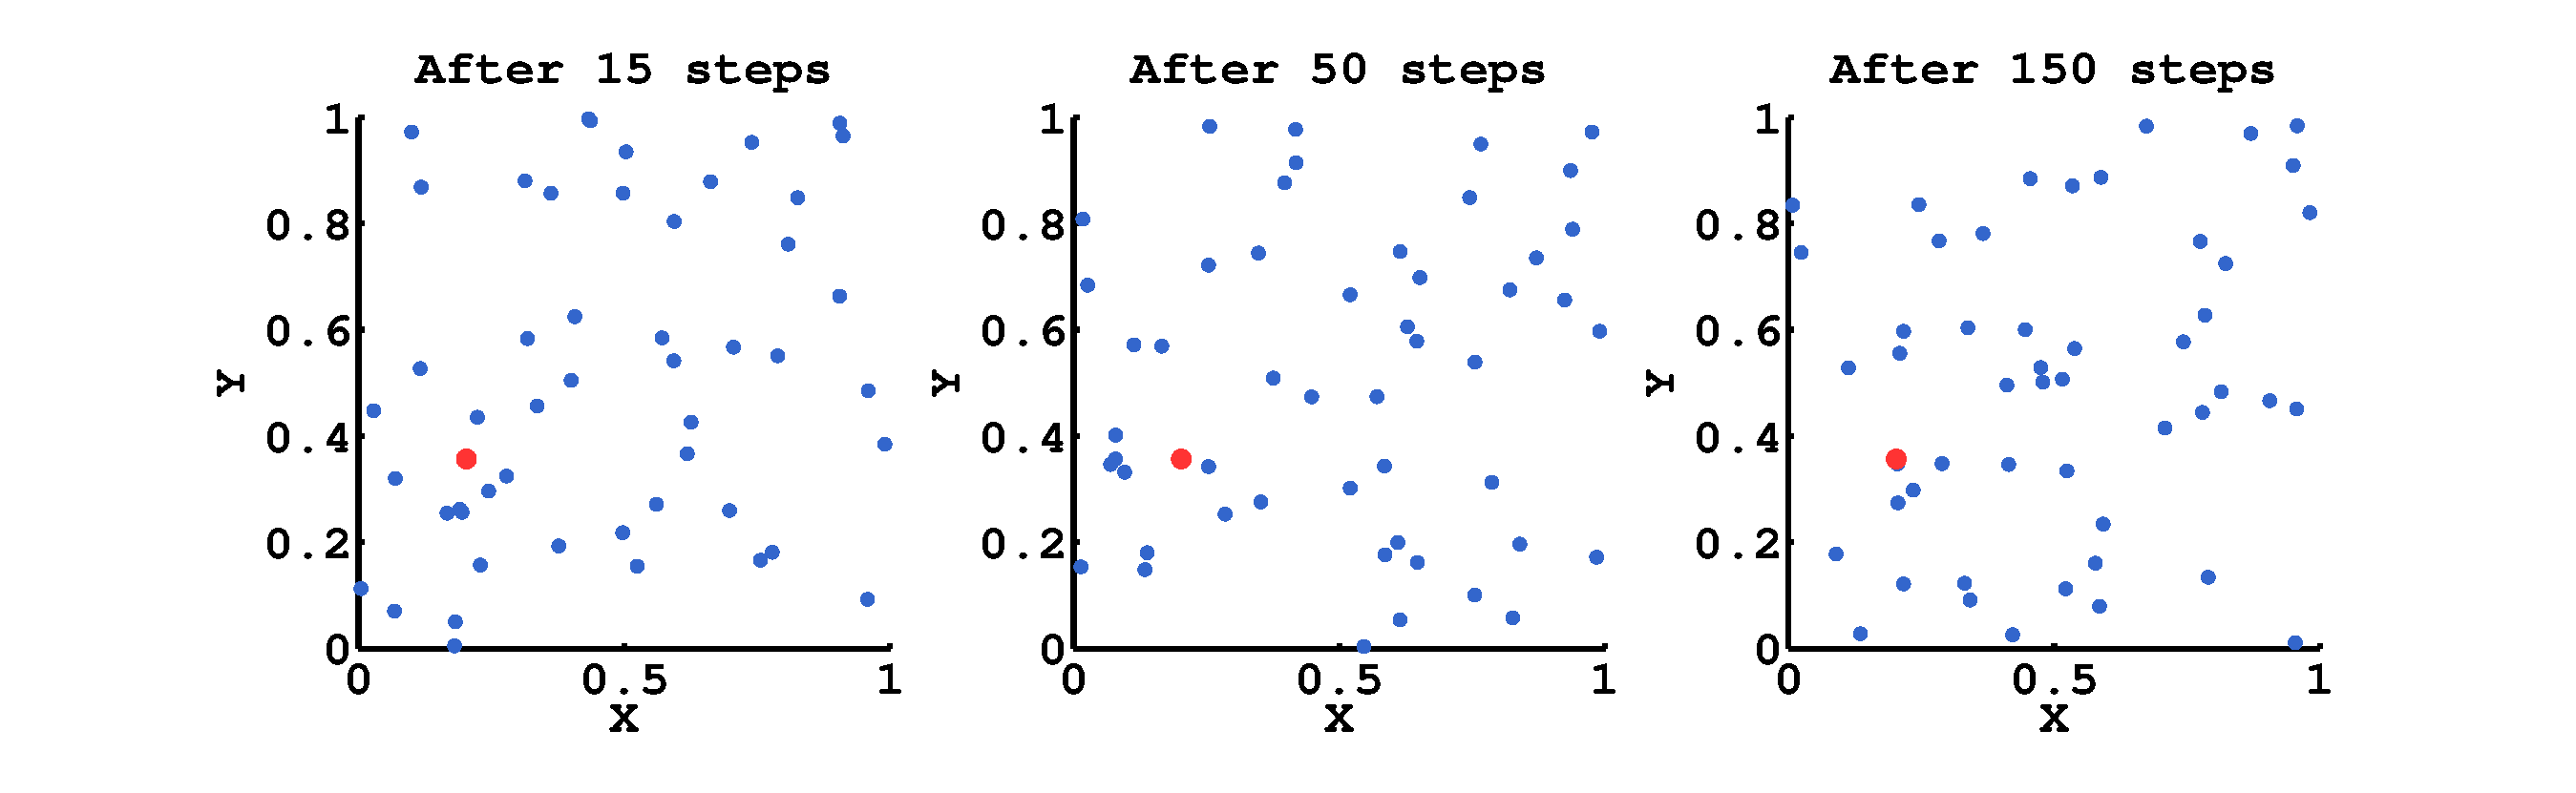
\includegraphics[width=\columnwidth, trim=3.5cm 0cm 3.5cm 0cm, clip=true]{\imgpath/continuous_task/maps/random_task_sampling.eps}
        \caption{Example of task hypothesis sampled using a random method.}
        \label{fig:continuoustaskrandomtask}
    \end{subfigure}
    \begin{subfigure}[b]{\columnwidth}
        \centering
        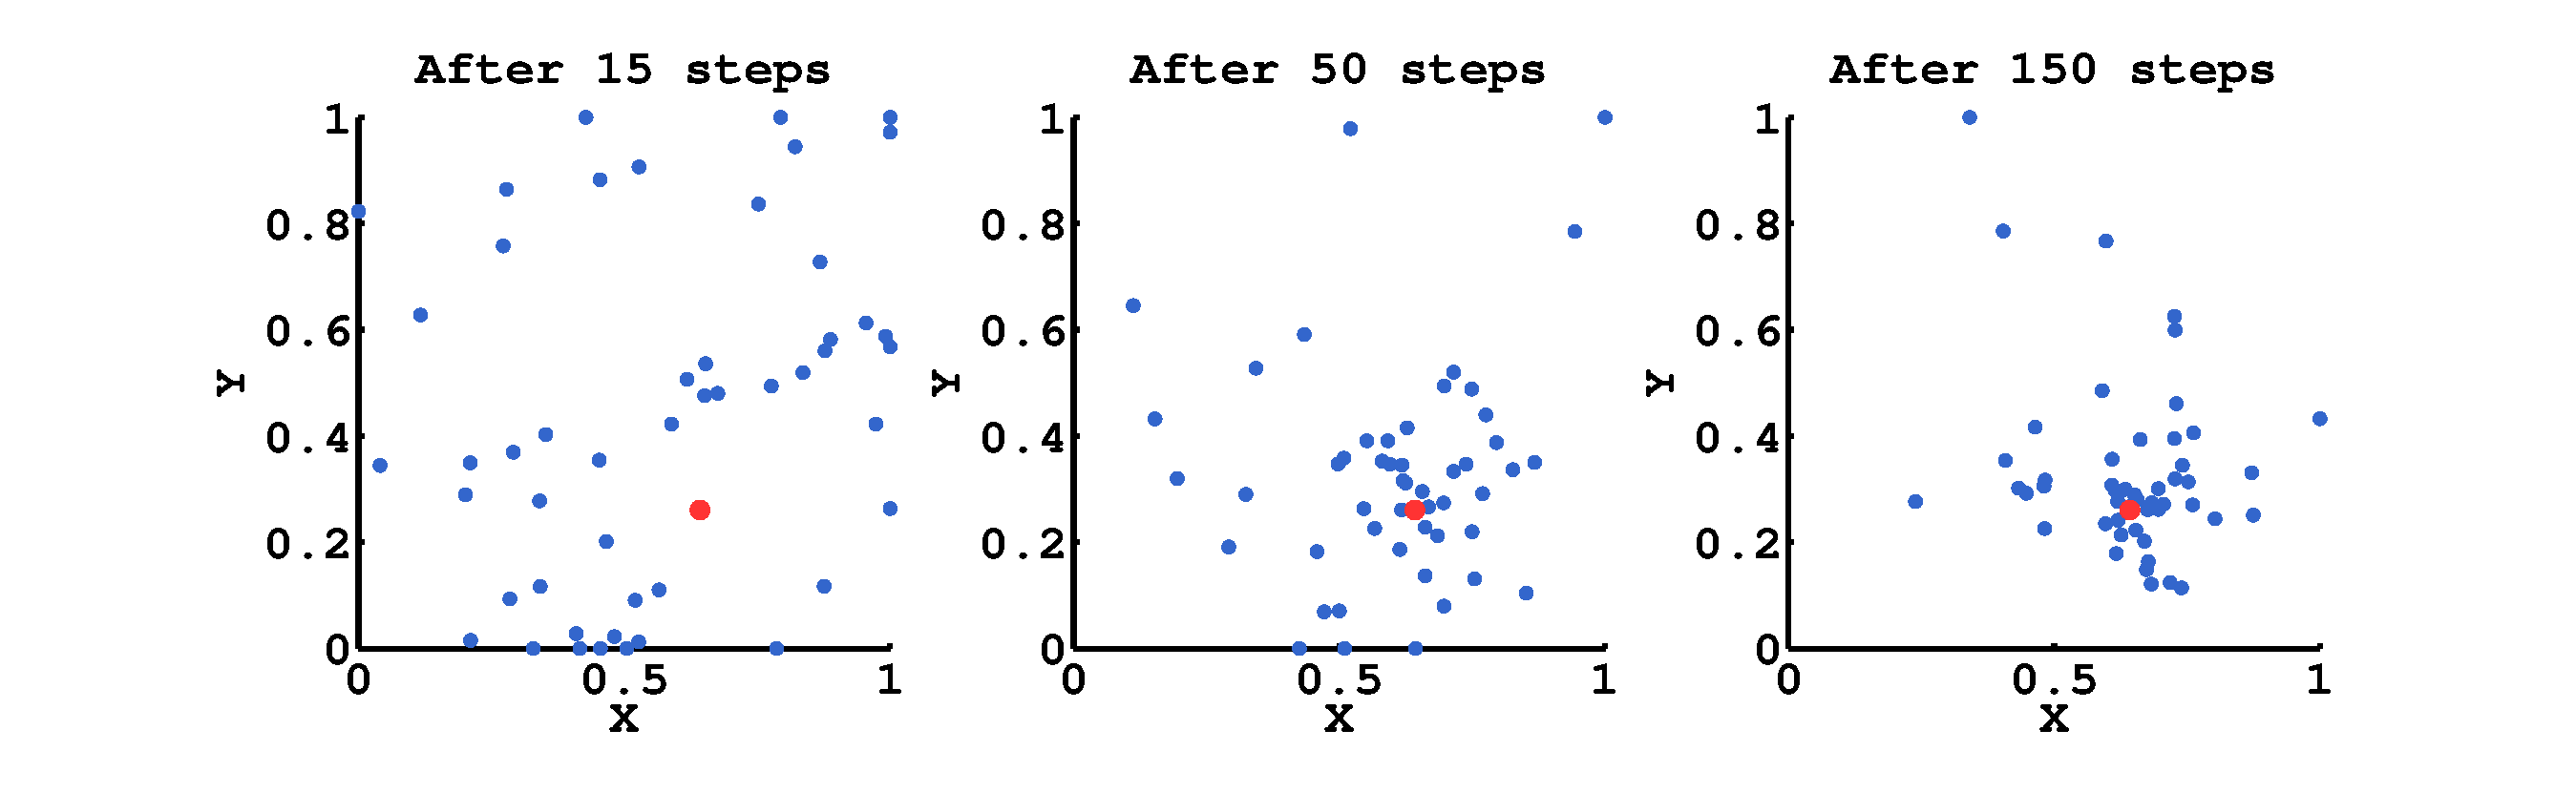
\includegraphics[width=\columnwidth, trim=3.5cm 0cm 3.5cm -1cm, clip=true]{\imgpath/continuous_task/maps/active_task_sampling.eps}
        \caption{Example of task hypothesis sampled using our active method.}
        \label{fig:continuoustaskactivetask}
    \end{subfigure}
\caption{Examples of task hypothesis sampling strategies. In red is the goal task. In blue are the sampled task hypothesis at iteration 15, 50 and 150. The active sampling method progressively focus his sampling around the goal state.}
\label{fig:continuoustasktasksampling}
\end{figure}

\paragraph{State sampling comparison}

We briefly illustrate the difference between our two state sampling methods, namely ``random'' and ``uncertainty''.

Figure~\ref{fig:continuoustaskstatesampling} shows the state visited (in blue) at after 200 steps  following a random (Fig.~\ref{fig:continuousstaterandomstates}) or an uncertainty based (Fig.~\ref{fig:continuousstateuncertaintystates}) next state selection method. The uncertainty based method allows to visit more states around the goal state (in red), which increases the changes of differentiates between the set of task hypothesis.

\begin{figure}[!ht]
\centering
    \begin{subfigure}[t]{0.49\columnwidth}
        \centering
        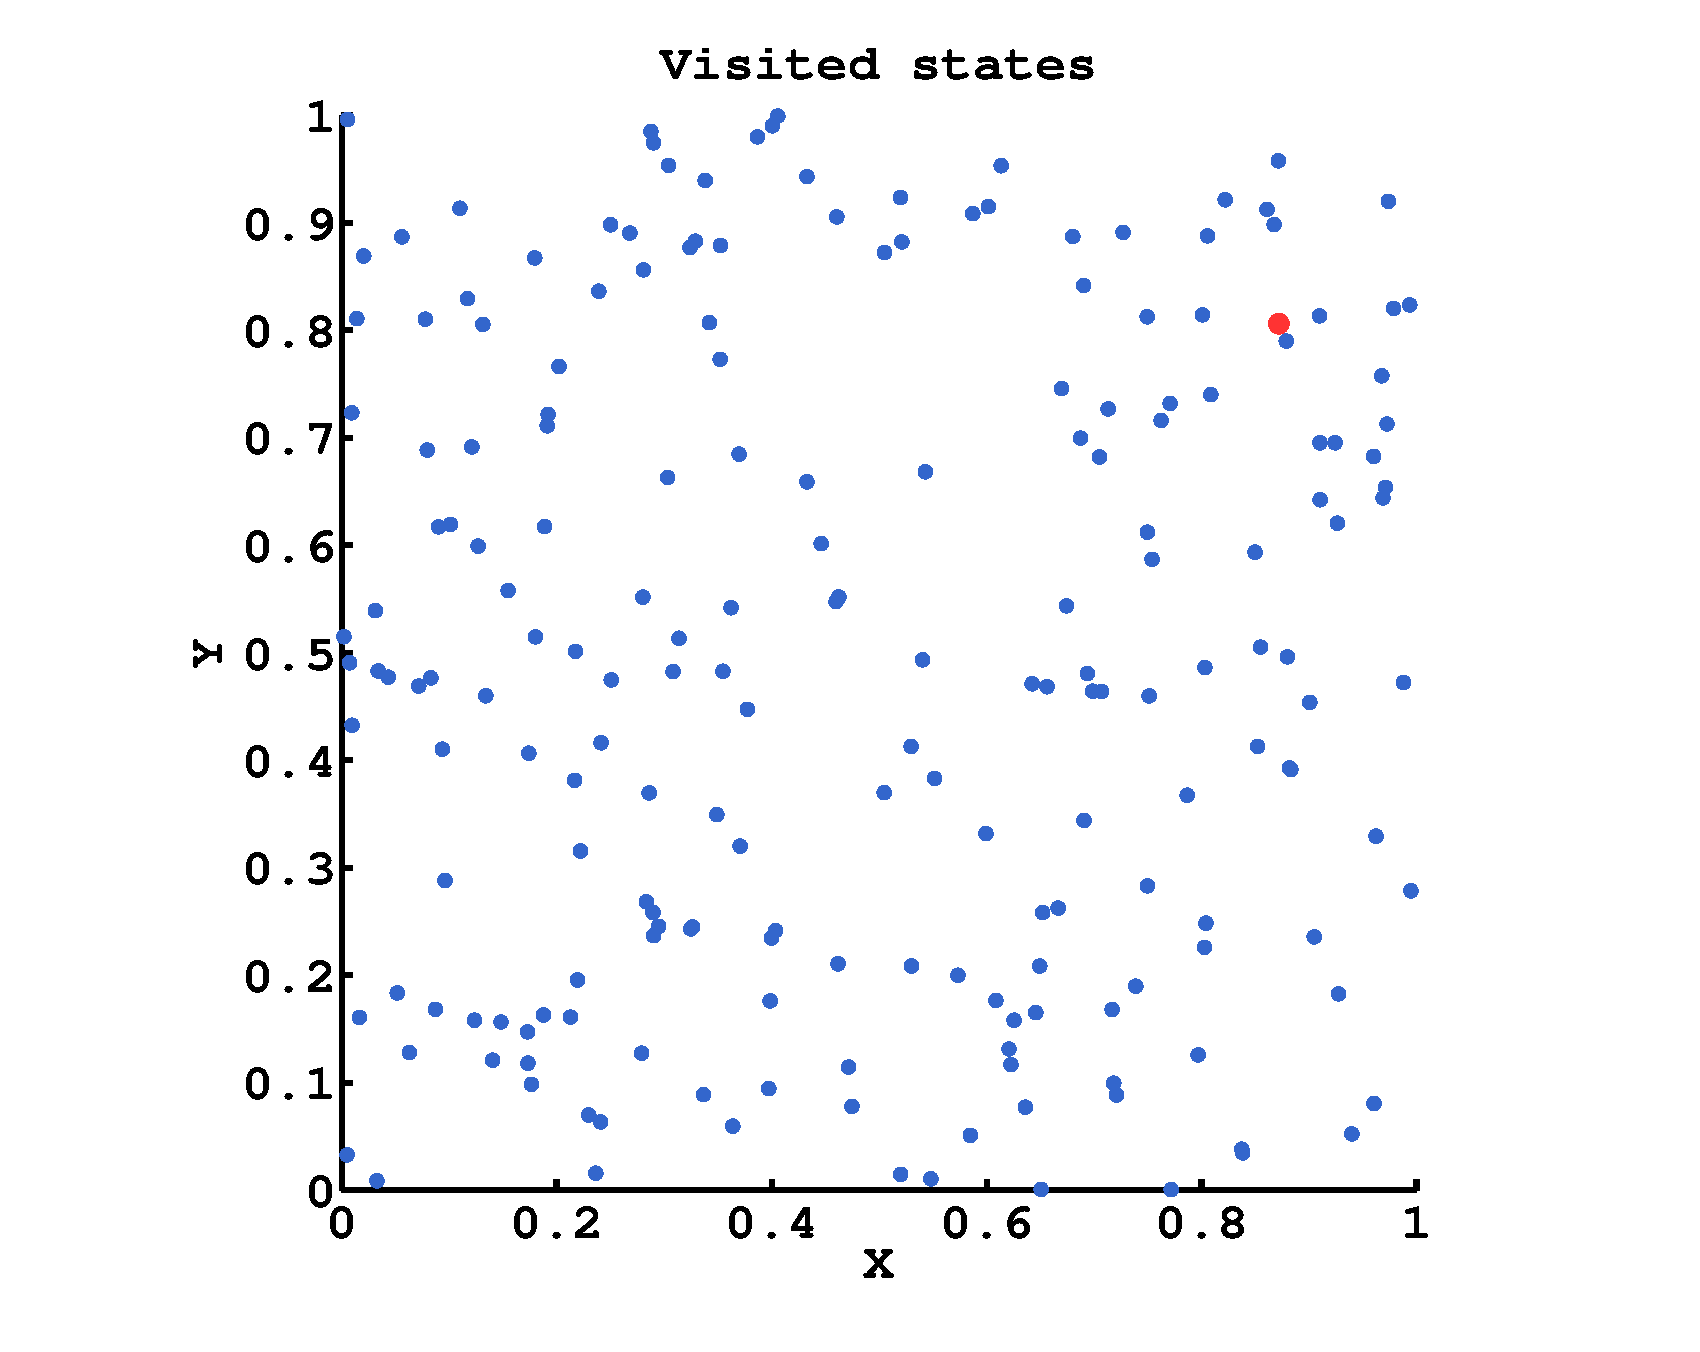
\includegraphics[width=\columnwidth, trim=2.5cm 0cm 2.5cm 0cm, clip=true]{\imgpath/continuous_task/maps/random_state_sampling.eps}
        \caption{Visited states after 200 steps with random state selection.}
        \label{fig:continuousstaterandomstates}
    \end{subfigure}
    \begin{subfigure}[t]{0.49\columnwidth}
        \centering
        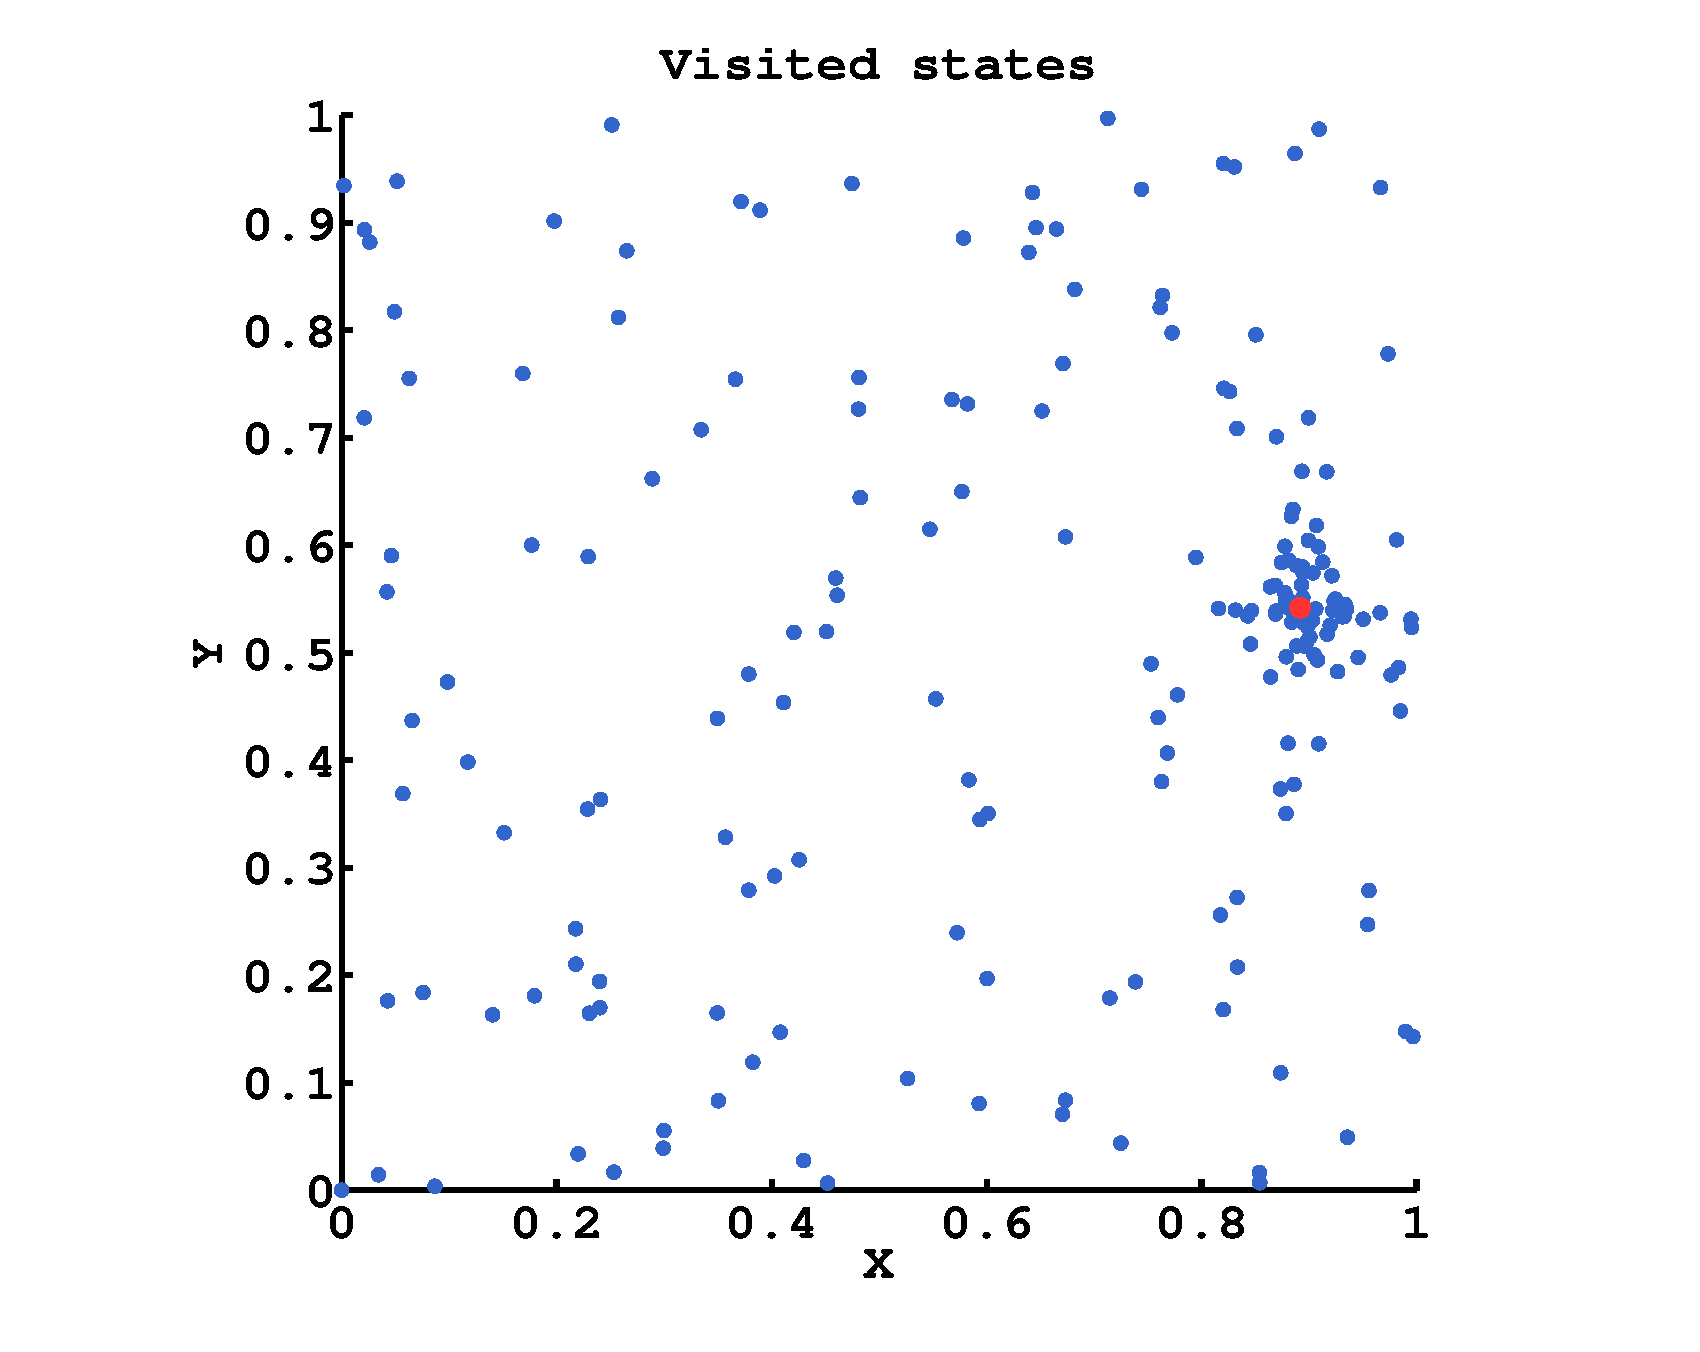
\includegraphics[width=\columnwidth, trim=2.5cm 0cm 2.5cm 0cm, clip=true]{\imgpath/continuous_task/maps/uncertainty_state_sampling.eps}
        \caption{Visited states after 200 steps with uncertainty based state selection.}
        \label{fig:continuousstateuncertaintystates}
    \end{subfigure}
\caption{The state visited by the agent, i.e. in which it received instruction signals, after 200 steps. In red is the goal task. Comparison of random state selection (left) and uncertainty based state selection (right). Selecting state according to their uncertainty, allow to collect more information around the goal state, which allow to identify more precisely the target location.}
\label{fig:continuoustaskstatesampling}
\end{figure}

Figure~\ref{fig:continuoustasktasksamplingexampleslow} details the uncertainty based method for selecting next visited states. Figure~\ref{fig:continuoustaskexampleslowdist} present the goal state for this specific run (right) and the evolution of the distance to the goal of the best estimate (left). Figure~\ref{fig:continuoustaskexampleslowweights} shows the set of task hypothesis at steps 15, 50, and 150 (as for Figure~\ref{fig:continuoustasktasksampling}) where the colors associated to each point represent the estimated probability of each task (red is high, blue is low). To sample the following agent's state, we sample 1000 states randomly and estimates the uncertainty of each of those point using the method described in chapter~\ref{chapter:planning} by Equation~\ref{eq:planning}. Computing this uncertainty requires to have a set of hypothesis and their associated weights (shown in Figure~\ref{fig:continuoustaskexampleslowweights}), access to the interaction frame and a classifier for each hypothesis. The resulting maps for step 15, 50, and 150 are displayed in Figure~\ref{fig:continuoustaskexampleslowuncertainty} where the colors represent the uncertainty values (red is high, blue is low). The less the distribution of probably on task is flat, the more the uncertainty map is narrow and focused around the best estimate. The active task resampling step is beneficial to the uncertainty state selection step as it allows to specify the uncertainty in key areas.

\begin{figure}[!ht]
\centering
    \begin{subfigure}[b]{\columnwidth}
        \centering
        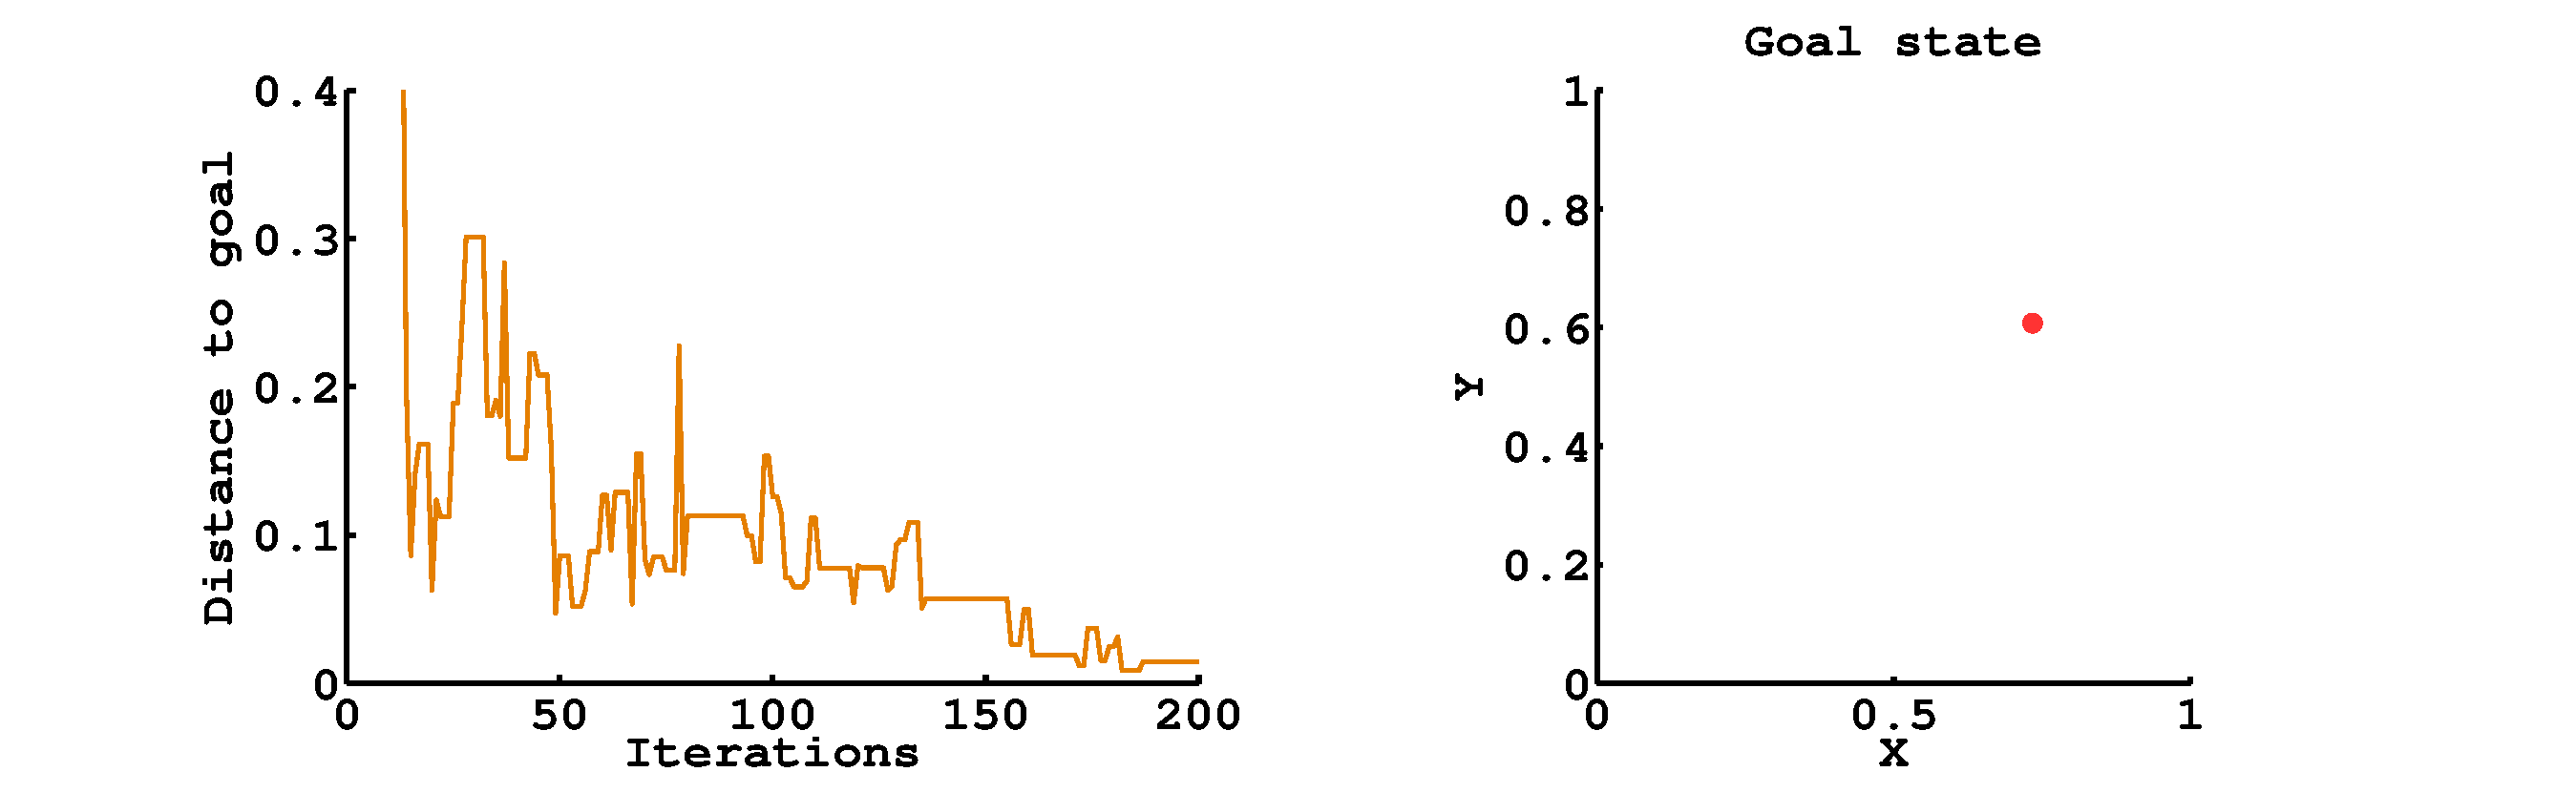
\includegraphics[width=\columnwidth]{\imgpath/continuous_task/maps/distgoal_slow.eps}
        \caption{Evolution of distance between he best task estimates and the goal position (left). The goal position being the red dot on the right plot.}
        \label{fig:continuoustaskexampleslowdist}
    \end{subfigure}
    \begin{subfigure}[b]{\columnwidth}
        \centering
        \includegraphics[width=\columnwidth, trim=2.5cm 0cm 2.5cm -1cm, clip=true]{\imgpath/continuous_task/maps/weights_slow.eps}
        \caption{Set of hypothesis after 15, 50, and 150 steps, with their associated probability show as colors. In order to allow for a good visualization of the maps, the associated value to each color are different for each time step. Red is associated to the most probable task, and blue for the less probable. The colors in the between are linearly maps according their associated weights.}
        \label{fig:continuoustaskexampleslowweights}
    \end{subfigure}
    \begin{subfigure}[b]{\columnwidth}
        \centering
        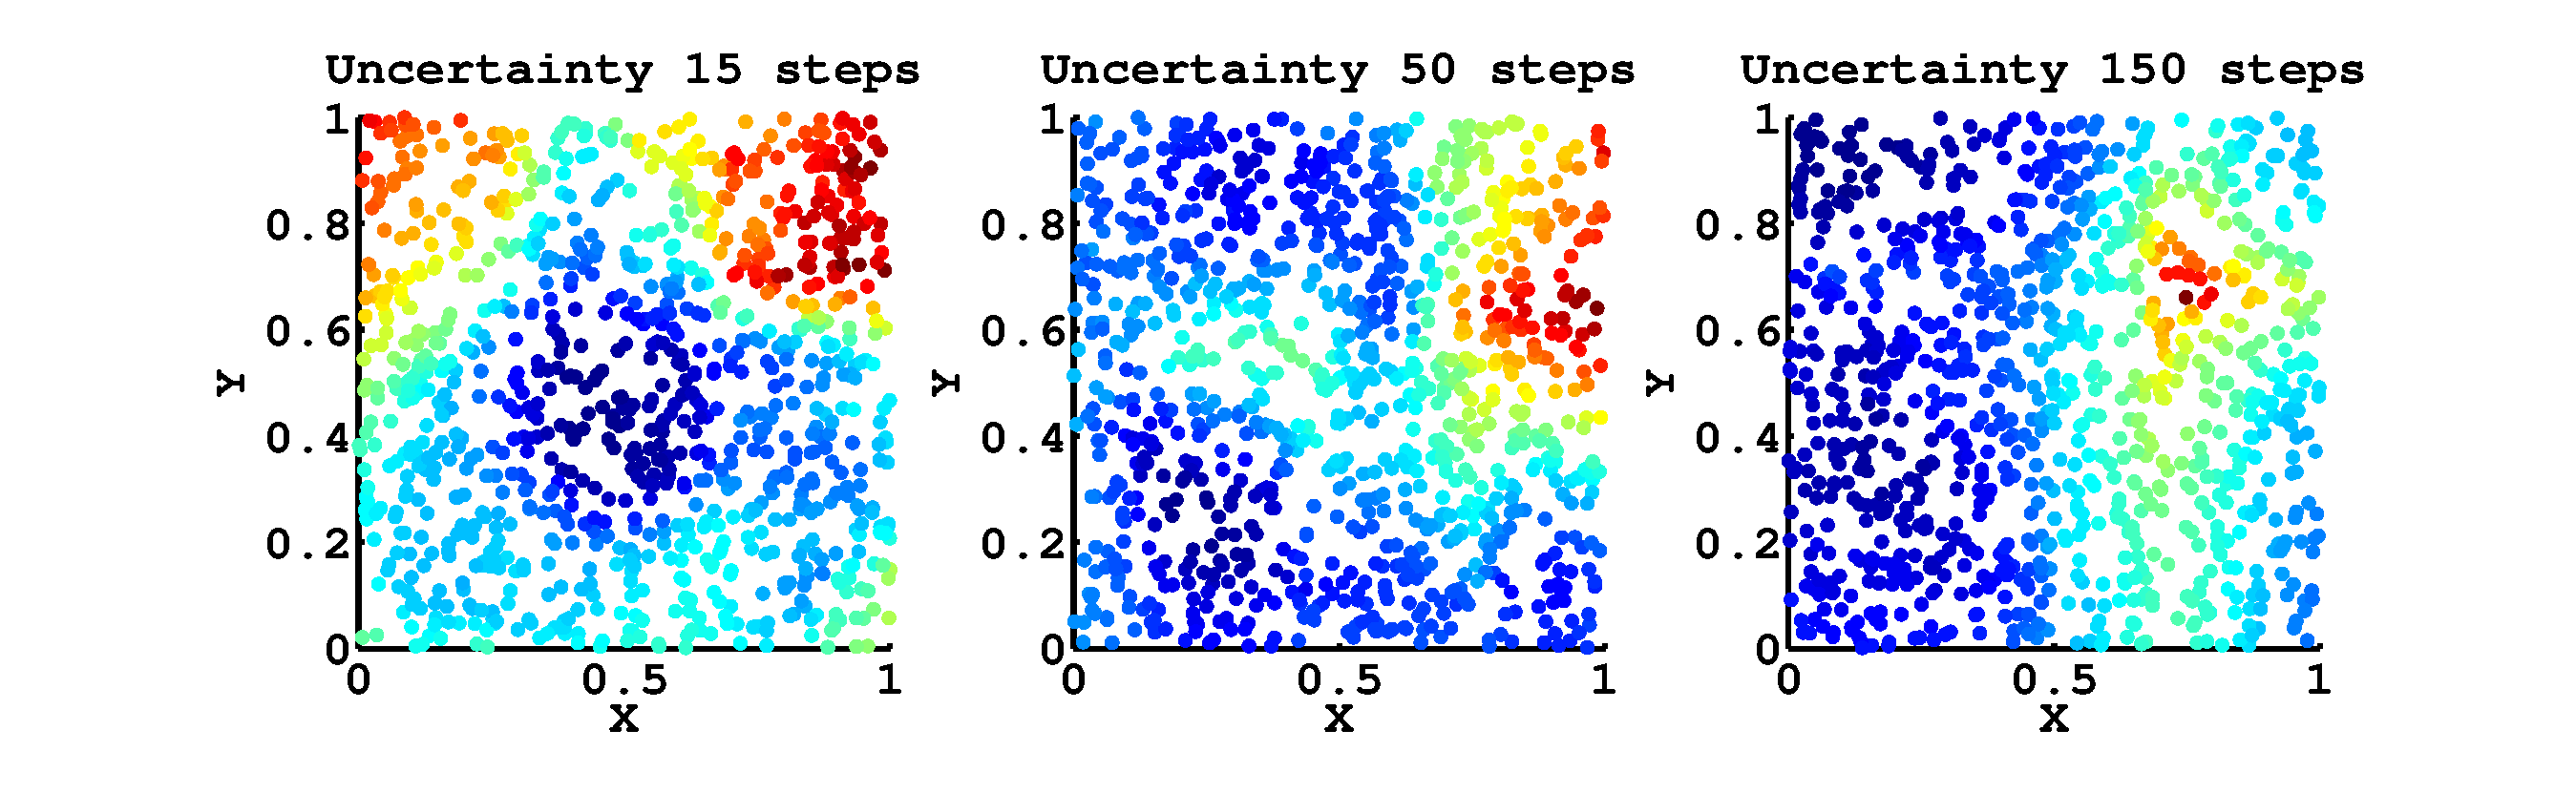
\includegraphics[width=\columnwidth, trim=2.5cm 0cm 2.5cm -1cm, clip=true]{\imgpath/continuous_task/maps/uncertainty_slow.eps}
        \caption{Uncertainty associated to each of the 1000 sampled states after 15, 50, and 150 steps. Only the most uncertain state will be select as the next state of the agent. The uncertainty maps evolve through time as the set of task hypothesis and their respective probability are updated. After 150 steps, the uncertainty is located around the goal position. In order to allow for a good visualization of the maps, the associated value to each color are different for each time step. Red is associated to the most probable task, and blue for the less probable. The colors in the between are linearly maps according their associated weights.}
        \label{fig:continuoustaskexampleslowuncertainty}
    \end{subfigure}
\caption{Illustration of the uncertainty based state sampling process after 15, 50, and 150 steps. The uncertainty is measure for 1000 randomly generated states and according to the current set of task hypothesis ans their associated probabilities.}
\label{fig:continuoustasktasksamplingexampleslow}
\end{figure}
